\documentclass[12pt]{article}
\usepackage[a4paper,left=1.25in,right=1.15in,top=1in,bottom=1in]{geometry}
\usepackage[T1]{fontenc}
\usepackage{mathptmx}
\usepackage{graphicx,booktabs,array,amsmath,amssymb,caption,subcaption,microtype,longtable}
\usepackage{float}
\usepackage[hidelinks]{hyperref}
\usepackage{xcolor}
\usepackage{authblk}
\setlength{\emergencystretch}{3em}
\captionsetup{font=small,labelfont=bf}
\renewcommand{\topfraction}{0.92}\renewcommand{\bottomfraction}{0.85}
\renewcommand{\textfraction}{0.06}\renewcommand{\floatpagefraction}{0.75}
\setcounter{topnumber}{3}\setcounter{totalnumber}{4}
\newcommand{\bp}{\,\text{bp}}
\graphicspath{{figs/}}

\title{\bf When the World Watches Football:\\[2pt] Bounds on the Aggregate Attention Channel and\\ the Limits of the World Cup Distraction Effect}
\author[1]{Daniel Gatto\thanks{Correspondence: \texttt{daniel@daru.finance}.}}
\affil[1]{Universidade Paulista (UNIP)}
\date{June 2026}

\begin{document}
\maketitle
\begin{abstract}
\noindent Ehrmann and Jansen show that when a country's team plays in the FIFA World Cup, the number of stock trades on that country's exchange falls by roughly half, an effect that runs through the local marginal trader who is also the local viewer. That mechanism is specific to a single national cash-equity exchange, and two distinct questions sit on top of it. One asks whether the synchronized \emph{global} attention shock depresses aggregate trading in markets that are continuous, global, derivative, or retail-heavy, where no national team maps to the marginal trader. A separate question, structurally closer to the original, is whether the \emph{local} distraction effect generalizes beyond its first venue. We separate them.

\smallskip\noindent Using one-minute data on eleven instruments across five market structures over the 2018 and 2022 tournaments, the aggregate channel is bounded near zero: during-match volume is statistically indistinguishable from zero in every market group, and equivalence tests reject the cash-equity literature's $30\%$ effect in every group, the deepest venues bounding it tightest (during-match volume declines beyond about $9\%$ excluded in crypto spot, $6\%$ pooled). These are genuine nulls rather than underpowered tests: injecting a known $30$--$45\%$ decline into the same panels, the estimator recovers it with essentially full power and correct size at the realized cluster counts.

\smallskip\noindent The local channel is harder, and we are explicit about why. The genuinely comparable object, a minute-level own-exchange trade count whose marginal trader is the local viewer, needs foreign intraday data that is not freely available; what we can test is CME own-currency futures (intraday, but a global marginal trader), US-listed country ETFs (intraday, but a US trader), and home equities for 26 nations (the right trader, but daily). None shows a decline, and the daily home response is bounded below about $11\%$, while the minute-level local effect Ehrmann and Jansen measured is left untested with power. The next-day loser effect of Edmans, Garc\'ia and Norli is absent at daily frequency in 20 national indices and 16 currencies.

\smallskip\noindent Our most transferable result is a pair of composition mechanisms by which two natural specifications manufacture the prior effect from no underlying response: a cross-market comovement decline ($-0.086$, $p=0.005$) that vanishes once the set of open instruments is held fixed, and an all-session cash-equity volume increase ($+19\%$) driven by extended-hours sampling. We do not claim to overturn the distraction effect in its own setting, which our evidence is consistent with; the contribution is the bound on the aggregate channel, the demonstration that the effect does not generalize to the venues that now carry the bulk of trading, and the two composition mechanisms.

\smallskip\noindent\textbf{Keywords:} investor inattention, limited attention, FIFA World Cup, trading volume, sports sentiment, loser effect, composition bias, equivalence testing, market microstructure.

\smallskip\noindent\textbf{JEL classification:} G14, G12, G15, G41, Z21.
\end{abstract}

\tableofcontents
\bigskip

\section{Introduction}\label{sec:intro}
The FIFA World Cup is among the largest synchronized attention events on earth, and the 2022 final drew a live audience in the hundreds of millions. Limited-attention theory predicts that an event this large pulls attention from markets and depresses trading while it runs \cite{barber2008,hirshleifer2009,dellavigna2009}. The sharpest evidence is Ehrmann and Jansen \cite{ehrmann2017}, who match minute-level trading on national stock exchanges to the World Cup schedule: when a country's team plays, the number of trades on that country's exchange drops sharply, by figures around $45$ to $55\%$ at the most attentive moments, with market activity ``following the ball.'' A separate strand documents sentiment rather than attention, where Edmans, Garc\'ia and Norli \cite{edmans2007} find a national index underperforms the day after the country loses an important match, and related work reports World-Cup-linked effects in US index returns and single-name sentiment \cite{kaplanski2010,bernile2011}.

That mechanism is specific. It runs through the marginal trader of a national cash-equity exchange, who in local daytime hours is disproportionately a local resident and therefore also the marginal football viewer. The same person sits on both sides of the distraction. The venue counts discrete trades, a measure sensitive to a thinning of small retail orders, and no substitute venue is open during the match. None of those features is shared by the markets that now carry most of the world's trading.

\paragraph{Two hypotheses.} That specificity splits the question in two, and the two need different tests. One concerns aggregate attention rather than any local trader:
\begin{quote}
$H_{\text{global}}$: the synchronized global attention shock depresses aggregate trading in continuous, global, derivative, or retail-heavy markets, where no national team maps to the marginal participant.
\end{quote}
A null in crypto, index, commodity, or currency futures bears on $H_{\text{global}}$, not on Ehrmann--Jansen, because a S\~ao Paulo viewer who stops trading during Brazil's match is a negligible share of global Bitcoin or S\&P-futures flow. The second hypothesis is Ehrmann--Jansen's own, carried to new venues:
\begin{quote}
$H_{\text{local}}$: the local distraction effect generalizes beyond the single national cash exchange to other mapped settings, where a team's own currency or home market is traded while the team plays.
\end{quote}
$H_{\text{local}}$ is the structurally comparable test, and it is the hard one. The genuinely matching object, a minute-level own-exchange trade count whose marginal trader is the local viewer, needs foreign intraday data that is not freely available.

\paragraph{What we find.} The attention shock is real and large; Wikipedia tournament-article views run $5.7\times$ and $8.0\times$ their baseline (Section~\ref{sec:attention}). The aggregate channel does not carry it. Across one-minute data on eleven instruments in five market structures, during-match volume is economically small and statistically indistinguishable from zero in every group, and equivalence tests reject a $30\%$ effect in every group while the deepest venues exclude declines beyond about $9\%$ in crypto spot and $6\%$ pooled (Section~\ref{sec:global}). A positive-control injection confirms the design recovers a $30$--$45\%$ effect with essentially full power at these cluster counts, so the nulls are informative rather than dead (Section~\ref{sec:robust}). On the local channel the bound reaches only as far as the available data. CME own-currency futures, US-listed country ETFs, and daily home equities all show no decline; the daily home response is bounded below about $11\%$; and the minute-level local-trader effect is left untested (Section~\ref{sec:local}). At daily frequency the next-day loser effect is absent in 20 national indices and 16 currencies (Section~\ref{sec:loser}). Two specifications reproduce the prior result as a composition artifact, the set of open instruments doing the work rather than any market response (Sections~\ref{sec:comov} and \ref{sec:loser}).

\paragraph{Contributions.} We bound $H_{\text{global}}$: the aggregate global attention shock does not move aggregate trading in continuous global markets, and we report how large an effect each venue excludes rather than asserting a bare null. For $H_{\text{local}}$ we offer a calibrated reading, since the distraction effect does not appear in any mapped venue we can reach but the precise Ehrmann--Jansen object is left untested with power; we therefore bound the daily home response and name the intraday foreign-exchange test as the open question rather than claiming a refutation in the original setting. Alongside the two hypotheses, we isolate two composition mechanisms by which natural specifications produce the prior finding from no underlying effect, the comovement case shown general with a Monte Carlo in which a zero-effect process produces a significant decline in $100\%$ of simulations.

\section{Related Work}\label{sec:related}
Three literatures meet at this paper. On \emph{limited attention}, the evidence is that attention is a
scarce resource whose diversion moves markets: Barber and Odean
\cite{barber2008} show retail buying concentrates in attention-grabbing stocks, DellaVigna and Pollet
\cite{dellavigna2009} find Friday earnings news is underreacted to because attention is low, Hirshleifer,
Lim and Teoh \cite{hirshleifer2009} document distraction by competing same-day news, and Da, Engelberg and
Gao \cite{da2011} validate search volume as a direct attention proxy. The World Cup is this literature's
cleanest natural experiment, a pre-scheduled attention shock with no confounding fundamental news.

A second strand applies that lens to football. Ehrmann and Jansen
\cite{ehrmann2017} are the direct antecedent and the result this paper tests: matching minute-level
national-exchange trading to the World Cup schedule, they find trade counts on a country's own exchange
fall by figures around $45$ to $55\%$ while its team plays, with attention ``following the ball.'' Edmans,
Garc\'ia and Norli \cite{edmans2007} document the sentiment counterpart, a next-day loser effect in the
losing nation's index, and Kaplanski and Levy \cite{kaplanski2010} and Bernile and Lyandres
\cite{bernile2011} report World-Cup-linked effects in US index returns and in single-name sentiment. What
this literature has not done is separate the aggregate-attention channel from the local-trader mechanism,
or test either outside the single national cash-equity exchange. Both findings rest on one venue, the
centralized daytime national exchange whose marginal trader is the local viewer, and neither has been
carried to the continuous, global, derivative, and retail-heavy venues that now intermediate most volume.

Methodologically the paper draws on an \emph{inference} toolkit the original event studies predate. We bound each
null with the two-one-sided-tests equivalence procedure \cite{lakens2017} rather than reading a
non-rejection as evidence of absence. The many-tests problem is handled with false-discovery control
\cite{benjamini1995}, and the count of nominal rejections is read against the multiple-testing critique of
empirical asset pricing \cite{harvey2016}. Where a cell rests on few match-day clusters we replace
asymptotic cluster-robust inference, which over-rejects in that regime, with the wild-cluster restricted
bootstrap of Cameron, Gelbach and Miller \cite{cameron2008}. The contribution relative to all three is to
split the World Cup question into a bounded aggregate channel and a power-calibrated local channel, and to
show that two natural specifications manufacture the prior finding through composition.

\section{Data and Sample}\label{sec:data}
\paragraph{Markets.} The core panel is one-minute data on eleven instruments in five market structures (Table~\ref{tab:universe}). Crypto bars come from \texttt{data.binance.vision} and carry dollar volume, trade count, and taker-buy volume; spot covers both tournaments and the perpetual enters in 2022. Futures one-minute trade bars come from AlgoSeek, front contract by daily volume, with quote-bearing TAQ for the liquidity tests and an end-of-day options-greeks feed from the same source. All core series are restricted to $\pm21$ days around each tournament so control minutes share the instrument's own regime. Because many matches fall on weekends, when futures are closed and crypto is the only open venue, the futures during-match sample concentrates in weekday and Sunday-Globex matches.

\begin{table}[h]\centering\small
\caption{The eleven core instruments span five market structures, chosen to differ from a national cash-equity exchange on the dimensions limited-attention theory says should matter.}\label{tab:universe}
\begin{tabular}{lll}\toprule
Group & Instruments & Structure \\\midrule
Crypto spot & BTC, ETH spot (Binance) & continuous, global, retail-heavy \\
Crypto perpetual & BTC, ETH USD\textsubscript{S}-M perpetual & continuous, leveraged, retail-heavy \\
Equity futures & ES, NQ (CME) & near-24h, institutional \\
Commodity futures & GC, CL (CME) & near-24h, global \\
FX futures & 6E, 6B, 6J (CME) & near-24h, automated \\
Cash equities & SPY, QQQ, IWM, 9 country ETFs & exchange-hours, the literature's venue \\\bottomrule
\end{tabular}
\end{table}

\paragraph{Home markets.} The local-channel arm (Section~\ref{sec:local}) adds three daily panels, the finest resolution freely available for foreign venues. Home equities for 26 nations (main index plus top-capitalization names, about 100 series, 2009--2023) come from the Yahoo Finance daily feed. Twenty national stock indices with deep history (1998--2022) and sixteen home currencies (each gated at its float or redenomination date: 1998 for the five developed units and South Korea, 2000--2007 for the rest, 2015 for the rouble) come from TradingView/ICE daily exports. Argentina's 1991--2001 dollar peg and the pre-2005 Turkish lira are excluded as untestable. Index returns are adjusted by the MSCI world return and currency returns are normalized to the dollar value of the local unit, so a negative return denotes home-currency depreciation.

\paragraph{Schedule, attention, controls.} Match results, kickoff times, and eliminations back to 1998 come from the Fjelstul World Cup database, with goal-level timing for 2010--2022. Attention is the daily Wikipedia tournament-article pageview series, with Google Trends and GDELT news volume as cross-checks. Estimation uses the completed 2010--2022 tournaments; the ongoing 2026 World Cup is excluded, though a live collector records it for a later out-of-sample extension.

\section{Identification}\label{sec:ident}
For instrument $i$ and minute $t$ we estimate
\begin{equation}\label{eq:main}
Y_{it} = \beta\, \mathrm{Match}_t + \alpha_{i,\,w(t)} + \gamma_{d(t)} + \varepsilon_{it},
\end{equation}
where $\mathrm{Match}_t$ is one during the in-play window of any match, $\alpha_{i,w(t)}$ is a fixed effect for instrument interacted with minute-of-week $w(t)$, and $\gamma_{d(t)}$ is a calendar-date fixed effect. The minute-of-week interaction compares a match minute to the same instrument at the same minute of the same weekday on non-match days, removing each instrument's intraday and weekly seasonality; the date effect absorbs whole-day shocks common across instruments. With the date effect included, $\beta$ is identified \emph{within} a calendar date, from the contrast between match and non-match minutes of the same day net of the minute-of-week seasonal: non-match days enter through the seasonal baseline they help estimate rather than as a direct cross-day comparison, so a quiet trading hour cannot masquerade as a match effect and a whole-day volatility or macro regime cannot leak into $\beta$. Standard errors cluster by calendar date, so the effective sample size for any treatment is the number of distinct match-days, not the number of minutes. The local-channel tests (Section~\ref{sec:local}) replace $\mathrm{Match}_t$ with an own-team indicator that is one only when the mapped nation's own team is playing. Outcomes are log volume, log trade count, absolute return, and the Parkinson high-low range \cite{parkinson1980}.

\paragraph{Power and bounds.} A null is informative only if the test could have caught a real effect. Each cell is reported with its $95\%$ confidence interval, the largest decline still consistent with the data, and the minimum detectable effect at $80\%$ power, then checked against a $30\%$ equivalence margin by two one-sided tests \cite{lakens2017}. Where a single market rests on very few match-day clusters, asymptotic cluster-robust inference over-rejects \cite{cameron2008}, so those cells are not flagged by assertion: each is re-tested with a wild-cluster restricted bootstrap (Frisch--Waugh residualization on the fixed effects and the foreign-match control, the null imposed, Rademacher cluster weights over match-days, $B=4999$), its bootstrap $p$ reported beside the asymptotic one (Section~\ref{sec:robust}). A well-powered cell's two $p$-values agree; a few-cluster cell's bootstrap $p$ inflates.

\paragraph{Pre-registration of the design.} The estimating equation, the clustering level, the $30\%$ equivalence margin, the primary-versus-exploratory split, and the rule that few-cluster cells are read through the bootstrap rather than the asymptotic $p$ are fixed before the cells are read. The 2026 tournament is held out of every estimate. Departures from a bare null, where they occur, are reported with the mechanism that produces them rather than corrected away.

\section{The attention shock is real}\label{sec:attention}
A null market response means nothing unless the attention shock is large, so we fix that first. Tournament-article Wikipedia pageviews run $5.7\times$ their off-tournament baseline in 2018 and $8.0\times$ in 2022, and the daily series tracks the match calendar, correlating $0.34$ and $0.70$ with the number of matches played that day. Figure~\ref{fig:attention} sets that spike beside the during-match volume response in the four no-mapping market groups: the left panel rises several-fold, the right sits on zero. Reconciling that gap occupies the rest of the paper.

\begin{figure}[h]\centering
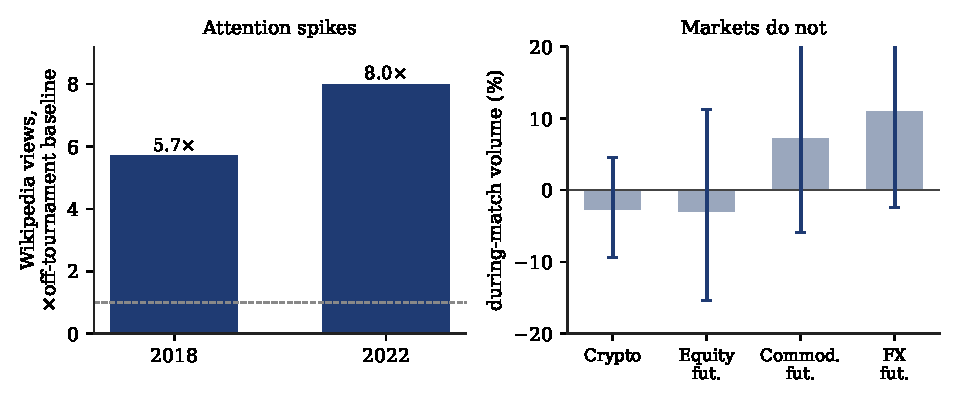
\includegraphics[width=0.92\linewidth]{fig_attention.pdf}
\caption{Attention spikes, the aggregate channel does not respond. Left: Wikipedia tournament-article pageviews as a multiple of the off-tournament baseline. Right: during-match change in trading volume for the four market groups with no national-team mapping, $95\%$ confidence intervals, all bracketing zero.}\label{fig:attention}
\end{figure}

\paragraph{The spike is intraday, not just a match-day average.} The daily
Wikipedia ratio could reflect heightened interest across the whole match-day rather than during the match
itself, which would leave open whether attention surges in the trading minutes the treatment isolates. The
Wikimedia hourly pageview dumps settle it at the during-match resolution, and we check three matches across
both tournaments rather than rest the point on one. Reconstructing each match hour by hour, the two
competing national-team articles and the tournament article jump in the kickoff hour against the same
articles three hours earlier. For the 2022 final (Argentina--France, kickoff $15{:}00$ UTC, 2022-12-18) the
tournament article runs $2.9\times$ ($5{,}245\to15{,}219$ views), Argentina's $3.3\times$
($1{,}038\to3{,}399$), France's $3.1\times$ ($893\to2{,}775$), and the Lionel Messi article $3.8\times$
($1{,}984\to7{,}582$), a mean of $3.3\times$ the pre-match baseline within the hour the match begins. The
pattern repeats: the 2018 final (France--Croatia) shows its two team articles at $3.0$ and $3.1\times$
(tournament article $1.7\times$, mean $2.6\times$), and the high-salience 2022 France--Morocco semifinal at
$2.2$ and $2.3\times$ (tournament $1.4\times$, mean $2.0\times$). Across the three matches the kickoff-hour
team-article spike runs $2.2$ to $3.3\times$ and never falls below $2\times$; the tournament article, already
elevated throughout the event, moves less for the non-final matches, as expected. The attention shock the
rest of the paper conditions on is present at the hour of play, not merely on the calendar day, so the
market nulls below are a non-response to a shock that is real at their own resolution.

\section{The aggregate global-attention channel}\label{sec:global}
$H_{\text{global}}$ asks whether the global attention shock depresses aggregate trading where no team maps to the marginal participant. It does not. Estimating Eq.~\eqref{eq:main} with log volume, the during-match change is $-2.7\%$ in crypto spot, $-3.9\%$ in crypto perpetuals, $-2.9\%$ in equity-index futures, $+7.2\%$ in commodity futures, and $+11.0\%$ in currency futures; pooled across all eleven instruments it is $+2.3\%$. None is significant, and the estimates are not consistently signed -- as compatible with a small increase as a small decrease, never the sharp decline distraction predicts. Table~\ref{tab:global} reports each cell with its interval and the decline it excludes. The bound is tightest in the deepest market: crypto spot, on 48 match-day clusters, rules out during-match volume declines beyond about $9\%$, and the pooled estimate rules out declines beyond about $6\%$. Equivalence tests against a $30\%$ margin reject an effect that large in every group. The bounds are not uniform, and we keep the gradient explicit rather than averaging it into one headline: crypto spot and the pooled estimate exclude declines beyond $9$ and $6\%$ and the $2.2$-million-minute quoted spread is pinned to $\pm1\%$, whereas the weekday-only futures cells are looser, ruling out only declines beyond about $15\%$ (equity-index futures) at a minimum detectable effect near $22\%$. The deep, continuously traded venues deliver precise nulls; the thinner cells deliver bounded ones. Figure~\ref{fig:bymarket} plots the same estimates against the $-30$ to $-50\%$ band the cash-equity literature reports; no interval reaches it.

\begin{table}[h]\centering\small\setlength{\tabcolsep}{6pt}
\caption{The aggregate global-attention channel ($H_{\text{global}}$). During-match change in trading volume by market group, with the largest decline still consistent with the data at $95\%$. Every interval brackets zero and the pooled estimate is positive; the marginal trader in each venue is global, not a national viewer.}\label{tab:global}
\begin{tabular}{lrrcr}\toprule
Market group & Effect (\%) & 95\% CI (\%) & Decline excl. & Clusters \\\midrule
Crypto spot (BTC, ETH)        & $-2.7$ & $[-9.4,\ 4.5]$  & $9\%$  & 48 \\
Crypto perpetual              & $-3.9$ & $[-16.2,\ 10.1]$& $16\%$ & 23 \\
Equity-index futures (ES, NQ) & $-2.9$ & $[-15.3,\ 11.3]$& $15\%$ & 31 \\
Commodity futures (GC, CL)    & $+7.2$ & $[-5.9,\ 22.2]$ & $6\%$  & 31 \\
FX futures, average match     & $+11.0$& $[-2.4,\ 26.3]$ & $2\%$  & 31 \\
\midrule
All instruments pooled        & $+2.3$ & $[-6.1,\ 11.5]$ & $6\%$  & 48 \\\bottomrule
\end{tabular}
\end{table}

\begin{figure}[h]\centering
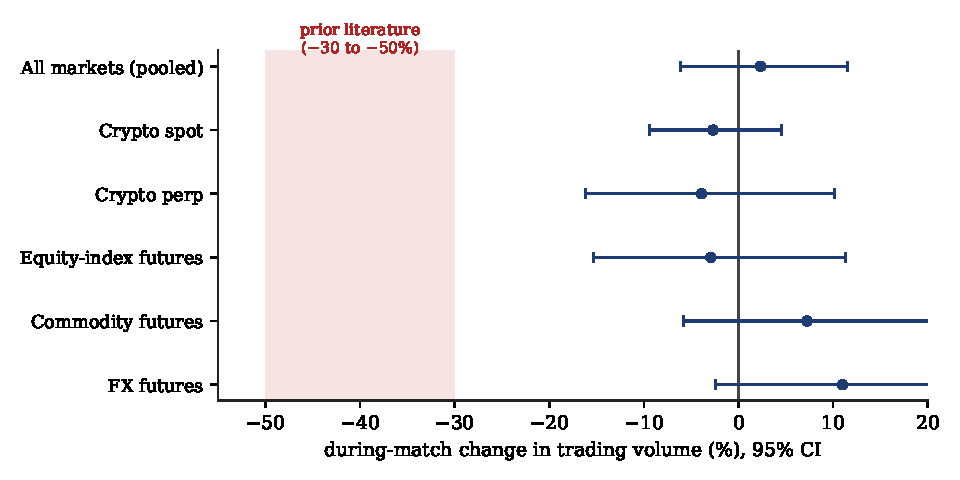
\includegraphics[width=0.86\linewidth]{fig_bymarket.pdf}
\caption{During-match volume by market group, $95\%$ confidence intervals, with the prior cash-equity literature's reported $-30$ to $-50\%$ decline shaded. No interval reaches the band; the pooled estimate is mildly positive.}\label{fig:bymarket}
\end{figure}

A minute-by-minute event study reaches the same place without the modeling. Figure~\ref{fig:kickoff} averages log volume in event time around kickoff across all matches: the series is flat through the opening whistle and across the $105$-minute in-play window, with no step at kickoff and no recovery at the close. A formal pre-trend check agrees, with eight pre-kickoff bins all insignificant (smallest $p=0.19$).

\begin{figure}[h]\centering
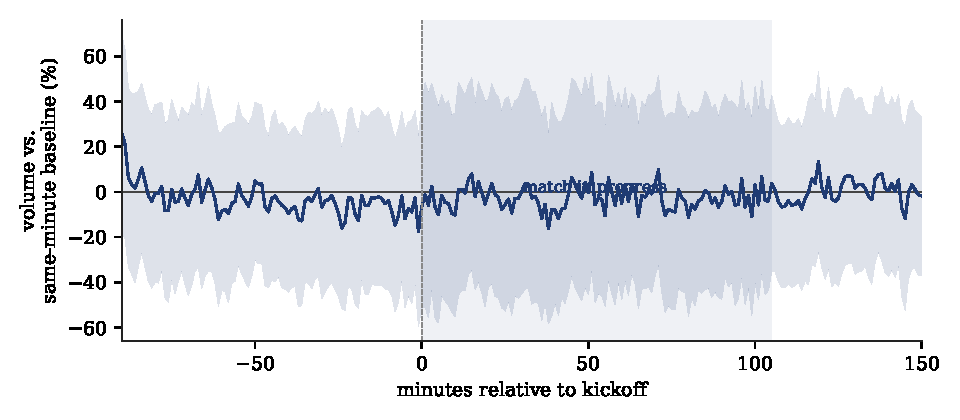
\includegraphics[width=0.9\linewidth]{fig_kickoff.pdf}
\caption{Trading volume in event time around kickoff, pooled across matches, relative to the same-minute-of-week baseline. The in-play window is shaded. Nothing steps at the opening whistle and nothing recovers at the close.}\label{fig:kickoff}
\end{figure}

Beyond volume, the liquidity and risk-pricing channels are equally flat. Across $2.2$ million instrument-minutes of bid/ask data, quoted spreads are unchanged ($+0.2\%$, $p=0.66$) and displayed depth is essentially flat ($-2.7\%$, $p=0.08$). At-the-money implied volatility and the 25-delta put-call skew do not move, option volume is flat, and variance ratios, the spot-futures and spot-perp bases, and lead-lag measures show no change in how quickly prices update.

\section{The ``comovement decline'' is a composition artifact}\label{sec:comov}
Where every direct channel came up flat, one specification reproduces the prior literature's effect, for a reason that generalizes. Computing the mean pairwise return correlation across all available instruments in match versus control windows, comovement falls during matches by $-0.086$ ($p=0.005$), the attention-driven decline the theory predicts. What moves is the set of instruments open during matches, not their correlation. Because many matches fall on weekends, the match-window correlation set tilts toward crypto, a higher-correlation cluster, relative to the weekday control set, so the mean correlation shifts on composition alone.

Two checks isolate the mechanism. Restricting to the constant crypto-only set that trades in both window types, the effect vanishes ($+0.012$, $p=0.54$); adding an instrument-count control to the full-sample regression does the same ($+0.002$, $p=0.93$). Figure~\ref{fig:comov}, left, shows only the naive estimate clears significance. The right panel establishes generality: in a Monte Carlo with an identical return process in match and control blocks and no match effect anywhere, letting only the set of contributing instruments differ across block types produces a spuriously significant comovement decline in $100\%$ of 400 simulations, which an instrument-count control returns to the nominal $5\%$. The spurious-rejection rate scales with the size of the composition shift; the $100\%$ shown is for a shift in the direction and rough magnitude of the weekend futures closures that drive the effect in our data, so it illustrates the mechanism's generality rather than fixing a single calibrated number. Holding composition fixed strips the raw-data confirmation back to nothing.

\begin{figure}[h]\centering
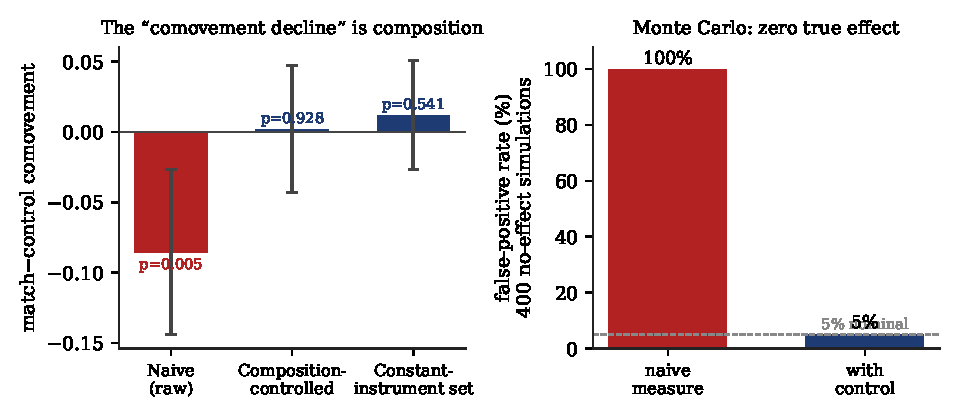
\includegraphics[width=\linewidth]{fig_comovement.pdf}
\caption{The cross-market comovement decline is composition, not attention. Left: the naive raw estimate is significant (red); holding the instrument set fixed or adding an instrument-count control returns it to zero. Right: a Monte Carlo with zero true effect and only a composition shift produces a significant decline in $100\%$ of simulations, and the control restores the nominal $5\%$ false-positive rate.}\label{fig:comov}
\end{figure}

\section{The local distraction channel}\label{sec:local}
Everything so far has tested the aggregate channel, where no national team maps to the marginal trader. We now turn to $H_{\text{local}}$, Ehrmann--Jansen's own hypothesis carried to new venues, the structurally comparable test and the hard one. The Ehrmann--Jansen object is a minute-level trade count on a national cash exchange whose marginal trader is the local viewer. No freely available data match all three of those features at once, so we test the cells that match two of them and read the result accordingly (Table~\ref{tab:local}). CME own-currency futures during the mapped nation's matches are minute-level but trade on a global, largely automated book rather than to local viewers. US-listed country ETFs during the home nation's matches are minute-level but trade to US investors. Home equities carry the right marginal trader but only at daily frequency.

\begin{table}[h]\centering\footnotesize\setlength{\tabcolsep}{4pt}
\caption{The local distraction channel ($H_{\text{local}}$): own-team effects in mapped venues. No cell matches all three features of the Ehrmann--Jansen object (minute-level, own home exchange, local marginal trader). Where the test is powered the estimate is positive or flat; the genuinely matching object is left untested.}\label{tab:local}
\begin{tabular}{lrrcc>{\raggedright\arraybackslash}p{1.7cm}}\toprule
Mapped own-team cell & Effect (\%) & 95\% CI (\%) & Clust. & Resol. & Marginal trader \\\midrule
Euro futures (6E), euro-area matches   & $+12.7$ & $[0.6,\ 26.2]$  & 60 & 1-min & global \\
Sterling fut.\ (6B), England matches$^{\dagger}$ & $-30.0$ & $[-44.0,\ -12.5]$ & 10 & 1-min & global \\
Yen futures (6J), Japan matches        & $+15.1$ & $[-7.3,\ 42.8]$ & 11 & 1-min & global \\
Own-team futures, pooled (2 tourn.)    & $+11.0$ & $[-4.0,\ 28.2]$ & 28 & 1-min & global \\
Own-team futures, pooled (4 tourn.)    & $+8.9$  & $[-3.9,\ 23.6]$ & 60 & 1-min & global \\
Country ETFs, own-country matches      & $-4.7$  & $[-17.2,\ 9.7]$ & 55 & 1-min & US \\
Home equities, own-match day           & $-0.6$  & $[-10.7,\ 10.7]$& 63 & daily & home (local) \\\bottomrule
\end{tabular}
\par\smallskip\footnotesize Marginal trader: \emph{global} = CME book, \emph{US} = US-listed ETF, \emph{home (local)} = the resident viewer (the Ehrmann--Jansen trader); only the last matches the original mechanism, and it is observed only at daily resolution. $^{\dagger}$ Ten match-days; date-clustered inference over-rejects at this cluster count \cite{cameron2008}, so this cell is not read as a finding.
\end{table}

Read across the table, no mapped cell shows a during-match decline, and the two best-powered cells are positive with intervals that exclude one. The euro-futures cell, on 60 own-match days, is $+12.7\%$ and its interval excludes any decline; the four-tournament own-team pool, also 60 clusters, is $+8.9\%$ and rules out declines beyond about $4\%$. The one large negative cell, sterling at $-30\%$, rests on ten match-days, exactly the regime where cluster-robust inference over-rejects,\footnote{Three sterling cluster counts appear in the paper, one per specification: the 2018--2022 own-team \emph{interaction} coefficient (six match-days, Section~\ref{sec:robust}), the four-tournament own-match \emph{level} cell reported here and in Table~\ref{tab:local} (ten), and the bootstrap specification on a marginally wider window (eleven, Table~\ref{tab:boot}). All three sit in the few-cluster regime and none is read as a finding.} and the per-nation cells conflict in sign (the yen $+15\%$, the peso $-21\%$, a meaningless Canadian-dollar $+91\%$ on two match-days). The home-equity cell carries the right marginal trader and shows $-0.6\%$ on 63 clusters, excluding a day-level home decline beyond about $11\%$.

What the table cannot do is see the Ehrmann--Jansen effect itself. That effect is a thinning of small trades during the match minutes on the team's own exchange. It can be present at minute resolution while averaging to nothing over a daily bar. Our minute-level mapped cells trade to global or US participants who do not watch the match, and our right-trader cell is daily. The minute-level own-exchange trade count with a local marginal trader is therefore the one test we cannot run, and we do not claim to have run it. Closing that gap needs intraday data for foreign cash exchanges, which is not freely distributed; it is the natural target for a paid-data extension.

\section{The next-day loser effect}\label{sec:loser}
Where the local distraction test ran into a resolution gap, its sentiment counterpart does not. The Edmans--Garc\'ia--Norli loser effect lives at daily frequency, its own native resolution, so here the evidence is direct. Across 20 national stock indices back to 1998 (110 match-day clusters), the first-session index return after the nation's own match, world-return adjusted, is $-0.5\bp$ after a loss ($p=0.96$); the developed-market subset shows $-15\bp$ ($p=0.14$) matched by an equal post-\emph{win} dip ($-10\bp$, $p=0.14$), so wins and losses are statistically indistinguishable and no loser effect is present. A placebo pins down what the common negative is not: the same nations' tournament-season index-days that are \emph{not} post-match sessions are flat ($+0.7\bp$, $p=0.87$, 205 date-clusters), so the post-match dip is specific to the session after a fixture rather than a season-wide calendar drift, and being equal for wins and losses it is in neither form a sentiment response to the result. The 16-currency panel back to 2002 (74 clusters) gives a next-session loser effect of $+9.9\bp$ ($p=0.13$), the opposite of what distraction predicts. Figure~\ref{fig:home} collects the home-market estimates; all bracket zero.

\begin{figure}[h]\centering
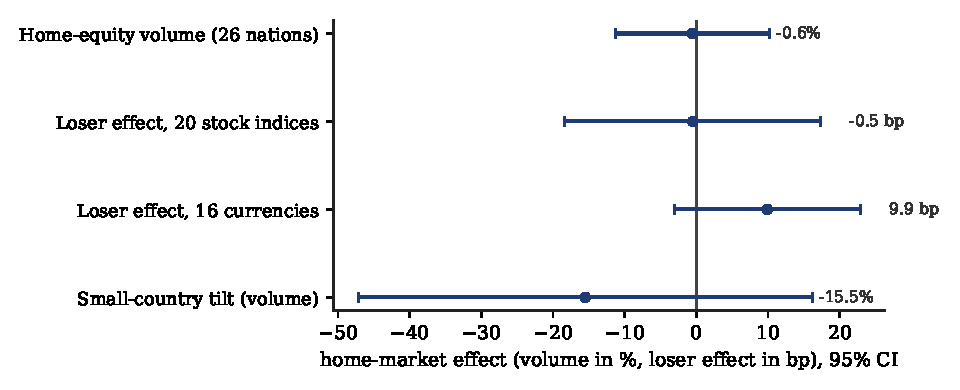
\includegraphics[width=0.86\linewidth]{fig_homemarket.pdf}
\caption{Home-market and home-currency effects, $95\%$ confidence intervals. Match-day home-equity volume, the next-session loser effect in 20 national indices and 16 currencies, and the small-country volume tilt all bracket zero.}\label{fig:home}
\end{figure}

Whether any effect should concentrate in the smallest, most retail-dominated economies is testable by interacting the own-match term with an emerging-market indicator, and the three measures conflict. Emerging-market home volume is $15\%$ lower on own-match days than the developed baseline ($p=0.30$, correctly signed but insignificant). The equity loser-effect interaction reverses sign and reaches nominal significance with the sign distraction does not predict ($+45\bp$, $p=0.05$, emerging markets falling \emph{less} after a loss), while the currency interaction is flat ($+3\bp$, $p=0.82$). A correctly signed but underpowered volume tilt in the smallest markets is the seam where a home effect could still hide, and only intraday foreign-exchange data could resolve it. A single-nation stand-alone test is not estimable in any case, which is the cluster-count point again: Brazil, the best case with 34 World Cup matches across six tournaments, has only six losses since 2002, and a return regression on six treated observations gives a degenerate standard error, so we report no single-nation loser-effect $p$-value.

Alongside the loser tests, the local-channel arm surfaces the second composition artifact. In US cash equities, the literature's own venue, regular-hours volume during matches is $-5.9\%$ ($p=0.19$) and trade count $-2.5\%$, both insignificant. A specification that adds thin pre- and post-market bars instead yields a spurious $+19\%$ trade-count increase ($p=0.02$), positive where distraction predicts a fall, and driven by when the sampled bars fall rather than by any market response.

\section{Robustness}\label{sec:robust}
The nulls survive the obvious stress tests. A placebo that shifts every match window forward one day is null, excluding minutes around scheduled macro releases leaves the estimates unchanged, and re-estimating at five- and fifteen-minute aggregation reproduces the one-minute figures. Widening the universe to 29 instruments across seven asset classes, adding the full Treasury complex, metals, energy, and more equity indices, produces two nominal rejections out of 29 against $1.5$ expected by chance, with a median absolute effect of $2.8\%$ and a dead-flat Treasury complex. High-stakes, knockout, and must-win matches show no larger effect than ordinary ones. Nor does the minute a goal is scored show a spike, against the in-play-betting intuition that informed flow should arrive there \cite{croxson2014}; the goal-window estimate is a marginally negative $\sim-7\%$ that holds steady across $\pm2$, $\pm5$, $\pm10$ and $\pm15$-minute windows and shifts by under half a point when the reconstructed goal timestamps are jittered by $\pm1$ to $\pm3$ minutes, so the absence of a spike is not an artifact of approximate goal timing.

The few single-market cells that look dramatic do not withstand inference, and each fails for a stated reason rather than a generic correction. Sterling-futures volume falls $34\%$ when England or Scotland plays and Nasdaq volume rises $35\%$ when the United States plays, but these rest on six and two match-days, the regime where date-clustered inference over-rejects \cite{cameron2008}. These are the 2018--2022 domestic-interaction coefficients (the differential against a no-mapped-team match); the four-tournament own-match \emph{level} cells in Tables~\ref{tab:local} and \ref{tab:boot} are smaller and rest on more match-days (sterling $-30\%$ on ten and $-23.5\%$ under the bootstrap on eleven, the one-day difference being the slightly wider window the bootstrap spec uses; Nasdaq $+16\%$ on eight, $p=0.40$), and every spec is read the same way. Pooled across mapped markets the own-team effect is a non-significant $+11\%$, positive where distraction predicts a fall. The comovement decline is composition (Section~\ref{sec:comov}), the all-session cash-equity jump is extended-hours sampling (Section~\ref{sec:loser}), and the per-currency cells conflict in sign on a handful of games each.\footnote{Pooling all 158 during-match and own-team coefficients the study produces, 19 are nominally significant at the $5\%$ level. We do not interpret this count as evidence for the null. The coefficients are nested and cross-correlated, so neither the binomial chance benchmark nor a false-discovery correction speaks to the hypotheses we argue; a Benjamini--Hochberg correction \cite{benjamini1995} removes all 19, but false-discovery control protects against false positives and does no work for a null thesis. The bounds in Tables~\ref{tab:global}--\ref{tab:local} and the per-cell mechanisms above carry the argument.}

\subsection{Few-cluster cells under the wild-cluster bootstrap}\label{sec:bootcells}
The claim that the dramatic single-market cells over-reject is itself testable. Table~\ref{tab:boot} re-runs the own-team cells with the wild-cluster restricted bootstrap of Section~\ref{sec:ident} beside the asymptotic cluster-robust $p$. The well-powered euro cell, on 59 own-match days, is unmoved: its asymptotic and bootstrap $p$ agree to the third decimal ($0.089$ versus $0.088$), so the positive euro estimate is not a small-sample artifact. The sterling cell, on eleven own-match days, behaves as the few-cluster regime predicts. Its $p$ roughly doubles under the bootstrap ($0.016$ to $0.031$), the asymptotic figure understating the true uncertainty. The two US cells are null on both. The bootstrap validates the inference rule: the asymptotic $p$ is trustworthy where clusters are plentiful and inflated where they are scarce. That is why the sterling and Nasdaq headline cells, even before the sign-conflict across currencies and the multiple-testing context, are read as low-cluster artifacts. The check is applied symmetrically, not only to the cells we dismiss: the pooled own-team cell we \emph{do} interpret sits at 28 clusters, and its asymptotic and bootstrap $p$ agree ($0.161$ versus $0.155$ all-mapped, $0.102$ versus $0.107$ FX-only), so the pooled $+11\%$ is not a small-sample artifact in either direction.

\begin{table}[h]\centering\small\setlength{\tabcolsep}{7pt}
\caption{Own-team volume cells under the wild-cluster restricted bootstrap ($B=4999$, Rademacher weights over match-days) beside the asymptotic cluster-robust $p$. The powered euro cell is unchanged; the few-cluster sterling cell's $p$ inflates; the US cells are null throughout; and the interpreted pooled cells (28 clusters) are stable across the two $p$-values.}\label{tab:boot}
\begin{tabular}{lrrrr}\toprule
Own-team cell & Match-days & Effect (\%) & $p$ (asy.) & $p$ (wild boot.) \\\midrule
Euro futures (6E), euro-area    & 59 & $+10.6$ & $0.089$ & $0.088$ \\
Sterling futures (6B), England  & 11 & $-23.5$ & $0.016$ & $0.031$ \\
Nasdaq futures (NQ), USA        & 8  & $+16.0$ & $0.398$ & $0.403$ \\
S\&P futures (ES), USA          & 8  & $-1.1$  & $0.950$ & $0.951$ \\
Own-team pooled, all-mapped     & 28 & $+11.0$ & $0.161$ & $0.155$ \\
Own-team pooled, FX-only        & 28 & $+14.9$ & $0.102$ & $0.107$ \\\bottomrule
\end{tabular}
\end{table}

\subsection{Could the design have caught the effect? A positive control}\label{sec:inject}
A null is only evidence if the test could have rejected. We never observe the Ehrmann--Jansen effect where it
is known to exist, so we inject it into our own panels and check recovery. For each headline cell we take the
real outcome residuals, add a known during-match decline of $-30\%$ or $-45\%$ (the prior literature's range),
and re-estimate with the same date-clustered inference; a zero injection returns the empirical size. Table~\ref{tab:inject}
reports the rejection rate over $B=2000$ draws. At the realized match-day cluster counts the well-powered cells
recover an injected $-30\%$ with power $1.00$ and correct $5\%$ size, and recover the coefficient without bias,
so their during-match nulls are informative, not dead tests. The single-market sterling design, on six
clusters, is the exception that proves the rule: its size is inflated to $0.11$ and its power against $-30\%$
falls to $0.75$, the same few-cluster fragility the bootstrap flags, which is why such cells are not read as
findings. One caveat scopes the recovery rates: the injection is a homogeneous multiplicative shift applied
to every match-minute, so these figures bound the design's power against a \emph{uniform} during-match
effect of the literature's size. An effect of the same average magnitude but concentrated in a minority of
matches would be recovered with less power, so the rates here are an upper bound; the well-powered cells'
nulls remain informative against the uniform effect the prior literature describes, which is the relevant
alternative.

\begin{table}[h]\centering\small\setlength{\tabcolsep}{7pt}
\caption{Positive-control injection. Empirical rejection rate at the $5\%$ level when a known during-match
effect is injected into the real panel, $B=2000$ wild-cluster draws at each cell's realized match-day cluster
count. The $0\%$ column is the empirical size; the $-30\%$ and $-45\%$ columns are power against the prior
literature's effect. Well-powered cells detect the effect with near-certainty; the six-cluster sterling design
loses size control.}\label{tab:inject}
\begin{tabular}{lrrrr}\toprule
Cell (design) & Clusters & Size ($0\%$) & Power $-30\%$ & Power $-45\%$ \\\midrule
Crypto spot (Match)            & 48 & $0.05$ & $1.00$ & $1.00$ \\
Equity-index futures (Match)   & 31 & $0.05$ & $1.00$ & $1.00$ \\
FX futures (Match)             & 31 & $0.05$ & $1.00$ & $1.00$ \\
Own-team futures, pooled       & 28 & $0.05$ & $1.00$ & $1.00$ \\
Sterling 6B, England (own)     & 6  & $0.11$ & $0.75$ & $1.00$ \\\bottomrule
\end{tabular}
\end{table}

\section{Discussion}\label{sec:disc}
The evidence answers the two hypotheses differently, and keeping them apart is what the data support. For $H_{\text{global}}$ the verdict is a clean, bounded no: the synchronized global attention shock, demonstrably real in the Wikipedia series, does not depress aggregate trading in continuous global markets, and the bound excludes declines a third the size of the cash-equity literature's in every venue. We do not oversell this. That the aggregate global attention shock would move global trading was no one's stated prior, so bounding it near zero is a useful negative rather than a surprise: a globally intermediated market does not depend on any one population's attention to keep trading, and flow a S\~ao Paulo viewer drops is absorbed elsewhere. Limited attention binds at the level of a person and of a local market; aggregate global liquidity does not register it.

$H_{\text{local}}$ admits a narrower reading. The distraction effect does not appear in any mapped venue we can reach, yet the venues that match Ehrmann--Jansen's resolution carry a marginal trader who is not the viewer, and the venue with the right trader is daily. We can bound the daily home response and we can say the effect does not show up in CME currency futures or US country ETFs, neither of which is traded by the distracted viewer. The original minute-level effect on a foreign cash exchange stays beyond reach, and our daily home-equity null is silent on an intraday dip that averages out over the session. What the data license is generalization-bounding, not refutation: the effect, real in its own setting, does not travel to the global and derivative venues that now dominate volume, and its survival at the minute level on a home exchange is left open.

Set beside those two verdicts on the football effect, the composition mechanisms carry a warning that outlasts it. Both the comovement and the full-session specifications are the kind of natural choice an author would make, and both produce the prior literature's effect from no underlying response. The Monte Carlo shows the comovement case is general: any cross-sectional comovement measure compared across windows that sample different instruments will show a spurious shift, and event windows that differ in their session mix will move any volume measure. Such artifacts survive most readily in an event-study literature that predates routine multiple-testing and composition checks.

\section{Threats to validity}\label{sec:limits}
Three limits frame the reading. Attention is validated at the daily level through Wikipedia and corroborated at the hour of play by the hourly Wikimedia reconstruction of three matches across both tournaments (Section~\ref{sec:attention}); finer attention within the during-match minutes themselves is inferred from television audience figures rather than measured directly. Because the exchanges close on Saturdays, the futures during-match sample tilts toward weekday and Sunday matches, and the cleanest weekend matches are observed mainly in crypto. The local-channel arm, in turn, is daily for the only cell with the right marginal trader, so it bounds the day-level home response and is silent on the intraday minutes the original cash-equity finding concerns. The first two limits qualify $H_{\text{global}}$ without undoing it, since the bound holds in venues open during weekend matches. The daily-resolution limit binds on $H_{\text{local}}$, and it is the reason we bound rather than refute.

\section{What would change the reading}\label{sec:deflate}
A reported null is worth only as much as the conditions that would overturn it, so we set those out. Two channels could in
principle weaken the $H_{\text{global}}$ bound. One is a mis-timing of the during-match windows against
the true kickoffs, but the minute-level event study (Figure~\ref{fig:kickoff}) is flat through the
opening whistle on the schedule we use, and the hourly attention reconstruction confirms the windows sit
where the attention is. The other is contamination of the matched control, against which the placebo, macro-
exclusion, and aggregation checks leave the estimates unchanged. The reading we cannot defend against
is the resolution gap on $H_{\text{local}}$. An intraday trade-count dip on a foreign cash exchange,
present at the minute and averaged away in our daily home bar, would be invisible to us. It is exactly the
Ehrmann--Jansen object, which is why we bound rather than refute it and why the paid intraday pull is the
decisive next step. Two things would change the headline if they appeared and have not. A powered own-team
cell turning significantly negative would revive $H_{\text{local}}$ in a mapped venue; instead the
best-powered comparable cell (euro futures, 60 match-days) is positive and survives the bootstrap
unchanged. A composition-robust comovement or session measure turning up the prior effect would
undercut the artifact claim; instead both vanish the moment the instrument set or the session window is
held fixed, and the Monte Carlo shows the naive versions manufacture the effect from nothing. The result
that would most cheaply falsify the whole paper, a clean during-match volume decline in any of the eleven
liquid global instruments, is not in the data.

\section{Conclusion}\label{sec:concl}
The World Cup is a clean, repeated, globally synchronized attention shock, and the markets that now carry most of the world's trading do not visibly respond to it in aggregate. During-match volume, volatility, liquidity, options pricing, and cross-market comovement are flat across crypto, index, commodity and currency futures, with equivalence bounds on volume and the quoted spread that exclude the declines the cash-equity literature reports (the volatility and options channels are reported as non-significant nulls without an equivalence margin), so the aggregate global attention channel is bounded near zero. The structurally comparable local test shows no decline in any mapped venue we can reach, the minute-level effect on a home exchange traded by local viewers is left untested with power, and the next-day loser effect is absent wherever daily data can test it. Both specifications that match the prior result turn out to be sampling which instruments or which session hours, not a market effect. The distraction effect, real in the national cash exchange where it was found, does not generalize to global, derivative and retail venues; whether it survives at the minute level on its own exchange is the question that paid intraday foreign data would settle.

\appendix
\section{Pre-registration}\label{app:prereg}
Fixed before the cells were read: the estimating equation~\eqref{eq:main}; clustering by calendar date;
the two-hypothesis split of Section~\ref{sec:intro}; log trade count as the primary $H_{\text{local}}$
outcome and log volume as the primary $H_{\text{global}}$ outcome; the $30\%$ two-one-sided-tests
equivalence margin; the rule that any cell on fewer than roughly thirty match-day clusters is read through
the wild-cluster restricted bootstrap rather than the asymptotic $p$; and the exclusion of the 2026
tournament from every estimate. The $H_{\text{local}}$ intraday verdict rule (reject if the pooled own-team
effect excludes $-30\%$; confirm if it is at or below $-30\%$ at $p<0.05$; otherwise report the achieved
bound) is registered in \path{HLOCAL_DATA_SCOPE.md} before any home-exchange data is acquired.

\section{Reproducibility}\label{app:repro}
The full pull-and-analysis pipeline is public at \url{https://github.com/DaruFinance/worldcup-attention-markets}; market data is not redistributed (AlgoSeek is licensed) but the scripts document every source and build step. Each result is produced by one script over the committed data, runnable offline. Every stochastic
procedure fixes its seed --- the comovement Monte Carlo, the wild-cluster and pooled bootstraps, and the
positive-control injection each pin a NumPy generator seed --- so the bootstrap $p$-values, the $100\%$
false-positive rate, and the injection power figures reproduce exactly on re-run. The control series for
the loser-effect adjustment (the MSCI-world ACWI and the dollar index) are cached to
\path{data/controls/} so the regressions reproduce bit-for-bit without a network call. Core analyses:
the cross-market and aggregate-channel tests (\path{analysis/reg_main.py}, \path{reg_bymarket.py}), the
equivalence and hypothesis split (\path{equivalence_tost.py}, \path{hypothesis_split.py}), the comovement
artifact and its Monte Carlo (\path{comovement.py}, \path{artifact_montecarlo.py}), the home-market and
loser-effect arms (\path{home_equities.py}, \path{equities_extended.py}, \path{fx_exotic_extended.py}),
the wild-cluster bootstrap on the single-market and pooled own-team cells (\path{wild_bootstrap.py},
\path{pooled_bootstrap.py}), the positive-control injection of Section~\ref{sec:inject}
(\path{injection_power.py}, emitting \path{injection_power.csv}), the loser-effect calendar placebo of
Section~\ref{sec:loser} (\path{loser_calendar_placebo.py}), the goal-window timing robustness
(\path{goal_timing.py}), the §\ref{sec:attention} intraday-attention
reconstruction of three matches across both tournaments (\path{attention_final.py}, emitting
\path{attention_hourly_final.csv} per article and \path{attention_hourly_matches.csv} per match from the
Wikimedia hourly dumps; \path{attention_hourly.py} is the vendor-slow pooled multi-match version), and
the global multiple-testing pool (\path{master_fdr.py}). The intraday
$H_{\text{local}}$ pipeline (\path{ingest/pull_home_intraday.py}, \path{analysis/hlocal_intraday.py}) and
its pre-purchase power calculation (\path{hlocal_feasibility.py}) are vendor-agnostic and run on a data
route when one is supplied.

\section{Figure and table provenance}\label{app:figs}
Figures are vector PDFs emitted by \path{paper/make_paper_figs.py} from the committed result CSVs in
\path{analysis/out/}: Figure~\ref{fig:attention} from \path{wiki_validation.csv} and
\path{equivalence_bounds.csv}; Figure~\ref{fig:bymarket} from \path{equivalence_bounds.csv};
Figure~\ref{fig:kickoff} from \path{kickoff_curve.csv}; Figure~\ref{fig:comov} from \path{comovement.csv}
and \path{artifact_mc.csv}; Figure~\ref{fig:home} from the home-equity, extended-index, and extended-FX
loser CSVs. Table~\ref{tab:global} is \path{equivalence_bounds.csv}; Table~\ref{tab:local} is
\path{fx_home_country.csv}, \path{pooled_domestic.csv}, \path{domestic_attention.csv}, and
\path{home_equities_distraction.csv}; Table~\ref{tab:boot} is \path{wild_bootstrap.csv}.

\section{Results inventory}\label{app:inventory}
The global multiple-testing pool (\path{master_fdr.csv}) holds all 158 during-match and own-team
coefficients across activity, liquidity, options, efficiency, comovement, intensity, goal windows,
sentiment, domestic, home-equity, home-currency, and breadth families; 19 are nominally significant, none
survives the global correction, and the smallest-$p$ cells are the mechanism-diagnosed artifacts named in
Section~\ref{sec:robust}. Equivalence bounds for every primary cell are in \path{equivalence_tost.csv} and
\path{equivalence_bounds.csv}; the two-hypothesis classification with per-cell bound, minimum detectable
effect, resolution, and marginal trader is in \path{hypothesis_split.csv}; the intraday $H_{\text{local}}$
feasibility table is \path{hlocal_feasibility.csv}.

\begin{thebibliography}{99}
\bibitem{ehrmann2017} Ehrmann, M., \& Jansen, D.-J. (2017). The Pitch Rather Than the Pit: Investor Inattention, Trading Activity, and FIFA World Cup Matches. \textit{Journal of Money, Credit and Banking} 49(4), 807--821. (Earlier as ECB Working Paper 1424, 2012.)
\bibitem{edmans2007} Edmans, A., Garc\'ia, D., \& Norli, \O. (2007). Sports Sentiment and Stock Returns. \textit{Journal of Finance} 62(4), 1967--1998.
\bibitem{kaplanski2010} Kaplanski, G., \& Levy, H. (2010). Exploitable Predictable Irrationality: The FIFA World Cup Effect on the U.S. Stock Market. \textit{Journal of Financial and Quantitative Analysis} 45(2), 535--553.
\bibitem{bernile2011} Bernile, G., \& Lyandres, E. (2011). Understanding Investor Sentiment: The Case of Soccer. \textit{Financial Management} 40(2), 357--380.
\bibitem{barber2008} Barber, B. M., \& Odean, T. (2008). All That Glitters: The Effect of Attention and News on the Buying Behavior of Individual and Institutional Investors. \textit{Review of Financial Studies} 21(2), 785--818.
\bibitem{da2011} Da, Z., Engelberg, J., \& Gao, P. (2011). In Search of Attention. \textit{Journal of Finance} 66(5), 1461--1499.
\bibitem{dellavigna2009} DellaVigna, S., \& Pollet, J. M. (2009). Investor Inattention and Friday Earnings Announcements. \textit{Journal of Finance} 64(2), 709--749.
\bibitem{hirshleifer2009} Hirshleifer, D., Lim, S. S., \& Teoh, S. H. (2009). Driven to Distraction: Extraneous Events and Underreaction to Earnings News. \textit{Journal of Finance} 64(5), 2289--2325.
\bibitem{croxson2014} Croxson, K., \& Reade, J. J. (2014). Information and Efficiency: Goal Arrival in Soccer Betting. \textit{Economic Journal} 124(575), 62--91.
\bibitem{benjamini1995} Benjamini, Y., \& Hochberg, Y. (1995). Controlling the False Discovery Rate: A Practical and Powerful Approach to Multiple Testing. \textit{Journal of the Royal Statistical Society B} 57(1), 289--300.
\bibitem{harvey2016} Harvey, C. R., Liu, Y., \& Zhu, H. (2016). $\ldots$ and the Cross-Section of Expected Returns. \textit{Review of Financial Studies} 29(1), 5--68.
\bibitem{lakens2017} Lakens, D. (2017). Equivalence Tests: A Practical Primer for $t$ Tests, Correlations, and Meta-Analyses. \textit{Social Psychological and Personality Science} 8(4), 355--362.
\bibitem{cameron2008} Cameron, A. C., Gelbach, J. B., \& Miller, D. L. (2008). Bootstrap-Based Improvements for Inference with Clustered Errors. \textit{Review of Economics and Statistics} 90(3), 414--427.
\bibitem{parkinson1980} Parkinson, M. (1980). The Extreme Value Method for Estimating the Variance of the Rate of Return. \textit{Journal of Business} 53(1), 61--65.
\end{thebibliography}

\end{document}
